% !TeX root = Main.tex

\section{Souvislost EMC a elektrické trakce} \label{sec:emc_trakce}
Elektrická trakce je velmi specifickou oblastí. Problematika elektromagnetické kompatibility je zde tak obsáhlá, neboť se týká nejen situace ohraničené prostorem vlakových souprav, ale i dalších propojených oblastí. Prolínají se tady elektrické systémy velice vysokých výkonů, nelineární výkonové elektronické prvky i systémy dopravní signalizační a zabezpečovací. Mezi konkrétní odlišnosti u~drážních zařízení patří například:
\begin{itemize}
\item topologie trakčního vedení (jednostranně nebo maximálně oboustranně napájené)
\item lokomotiva představuje jednofázovou zátěž o~značném výkonu v~řádech MW \footnote{např. ŠKODA 109 E disponuje jmenovitým výkonem 6400 kW}
\item proměnná vzdálenost mezi napájecí stanicí a místem odběru (s~tím související variabilita parametrů vedení)
\end{itemize}
Dle \cite{emc_trakce} je na problematiku EMC v~elektrické trakci nahlíženo komplexně a rozděluje se dle kmitočtových pásem na 2 oblasti:

\medskip
{\bf Nízkofrekvenční rušení} - frekvenční pásmo 0 až 2500 Hz \\
Zdroje rušení představují především polovodičové měniče. Ty během své činnosti vytvářejí vyšší harmonické proudy. Vzhledem k~rozsahu provozovaných výkonů se jedná o~nezanedbatelnou složku v~trakčním napájecím vedení. Důsledkem tohoto typu rušení je zvýšení odběru jalového a deformačního výkonu, čímž dochází k~souvisejícímu zhoršení celkového účiníku $\lambda$ (často označovaný jako \uv{power factor}). Vliv vyšších harmonických nelze nikdy úplně odstranit, ale lze snížit jejich účinky. To se týká především omezením velikostí proudů konstrukcí měničů, metodami řízení, doplňkovou výbavou či dalšími kompenzačními zařízeními a filtry. O~daných prostředcích blíže pojednává~\cite{nfr}.

\medskip
{\bf Vysokofrekvenční a impulsní rušení} - frekvenční pásmo 9 kHz až 1 GHz \\
V~této kmitočtové oblasti jsou předmětem zájmu impulsy, které vznikají při spínacích pochodech v~napájecích stanicích, případně i v~lokomotivách. Zdroje tohoto rušení mohou nepříznivě až kriticky ovlivňovat kromě všech drážních zařízení také blízké okolí rozvodů trakčního vedení. Mezi obzvláště citlivé spotřebiče na rušivé vlivy od elektromagnetického pole lze považovat zařízení komunikací, sdělovací systémy a veškerá řídící technika, realizovaná v~dnešní době procesorovou a číslicovou elektronikou. O~úrovních přípustného rušení v~elektrické trakci je pojednáno v~příslušných normativech, které jsou popsány v~podkapitole \ref{sec:emc_normy_trakce}. Omezení vlivu elektromagnetického pole na dané zařízení je možné pomocí stínění, k~jehož návrhu a realizaci je čato vhodné využití simulačních aplikací. Více o~tom pojednává kapitola \ref{kap:Simulace}.
\newpage

\section{Struktura norem EMC}
EMI interference, EMS susceptibilita
\newpage

\section{Aktuální normativy v~elektrické trakci} \label{sec:emc_normy_trakce}
Mezi aktuální normy, související s~elektromagnetickou kompatibilitou v~elektrické trakci, patří především České technické normy s~označením ČSN EN 50121. Jedná se o~překlady, které zajišťuje Český normalizační institut. Mají proto stejný statut jako oficiální verze, kterými jsou evropské normy EN 50121, vydávané Evropským výborem pro normalizaci v~elektrotechnice (CENELEC). 

 Z~řady důvodů, uvedených v~podkapitole \ref{sec:emc_trakce},  je elektromagnetická kompatibilita vážným problémem již při konstrukci a výrobě trakčních vozidel. Proto je nutné vytvořit normy, které budou splňovat jak veškeré požadavky Směrnice elektromagnetické kompatibility EC 89/336/EEC, tak i zajišťovat spolehlivost a funkčnost vlastních drážních zařízení.

Soubor norem ČSN EN 50121, vydaný pod společným názvem Drážní zařízení – Elektromagnetická kompatibilita, je rozčleněn na šest logicky souvisejících částí. Bylo by neúčelné vypisovat veškerá specifika, tabulky a grafy, které jsou v~těchto normách uvedené, proto se budu snažit zaměřit pouze na hlavní oblast zájmu, kterého se daný normativ týká. Přesnější informace je možné získat nahlédnutím do příslušného dokumentu. \bigskip \\
Část 1: Všeobecně\\
Část 2: Emise celého drážního  systému do vnějšího prostředí\\
Část 3-1: Drážní vozidla – Vlak a celkové vozidlo\\
Část 3-2: Drážní vozidla – Zařízení\\
Část 4: Emise a odolnost zabezpečovacích a sdělovacích zařízení\\
Část 5: Emise a odolnost pevných instalací a zařízení trakční napájecí soustavy\\

\subsection{ČSN EN 50121-1}
Norma ČSN EN 50121-1: Všeobecně popisuje rozdělení celého vlastního souboru norem, jak je uvedeno výše. Dále obsahuje postupy pro řízení managementu pro dosažení EMC v~elektrické trakci. Nakonec především stanovuje funkční kritéria, které jsou založeny na evropské normě EN 61000-6-2. S~jejich pomocí se posuzuje funkčnost a schopnost provozu zařízení během zkoušek EMC. V~normě jsou popsána 3 funkční kritéria, označovaná jako A, B a C. Pokud testovaný vzorek není schopen splnit požadavky alespoň jednoho z~uvedených kritérií, posuzuje se jako nevyhovující.

Funkční kritérium A~ve většině případů nedovoluje žádnou změnu chování zařízení během i následně po skončení zkoušek EMC. Jedinou modifikací může být výrobcem nastavená minimální hranice fungování, případně přípustná mez ztráty funkčnosti, které přesto výrobek během i po testech nesmí překročit.

Funkční kritérium B opět nedovoluje zhoršení funkce, pokud je zařízení používáno podle svého určení, avšak pouze po ukončení zkoušek. Během testů je akceptovatelné zhoršení činnosti za předpokladu, že se nezmění současný provozní stav a nedojde ke ztrátě dat v~paměti zařízení.

Funkční kritérium C popisuje, že u~zkoušeného zařízení je možná dočasná ztráta funkce, pokud je nějakým prostředkem možno zajistit její obnovení.

\subsection{ČSN EN 50121-2}
Norma ČSN EN 50121 - 2: Emise celého drážního  systému do vnějšího prostředí ustanovuje mezní hodnoty emisí, které mohou být produkovány při provozu drážních vozidel. Dále určuje, jakým způsobem měření lze dané hodnoty ověřit. Dle normy se předpokládá, že elektromagnetické rušení, působené elektrickou trakcí, existuje ve všech místech ve vzdálenosti 10 m od vnější elektrizované troleje nebo 10 m od trakční napájecí stanice. Proto je i stanoveno provádět měření emisí v~této vzdálenosti. Pokud není možné tuto podmínku vzhledem k~místním poměrům na dráze dodržet, existuje v~normě definovaný přepočet pro měření v~jiné ekvivalentní vzdálenosti. 

Mezní hodnoty se podle normy rozlišují na vyzařování z~venkovní dráhy při provozu vlaku a samostatně na emise z~trakčních napájecích stanic. Hranice (velikost vrcholové hodnoty) pro jednotlivé napájecí systémy v~elektrické trakci používané v~České republice jsou uvedeny v~grafu na obrázku \ref{obr:emc_emise}.

\begin{figure}[!h]
	\centering
	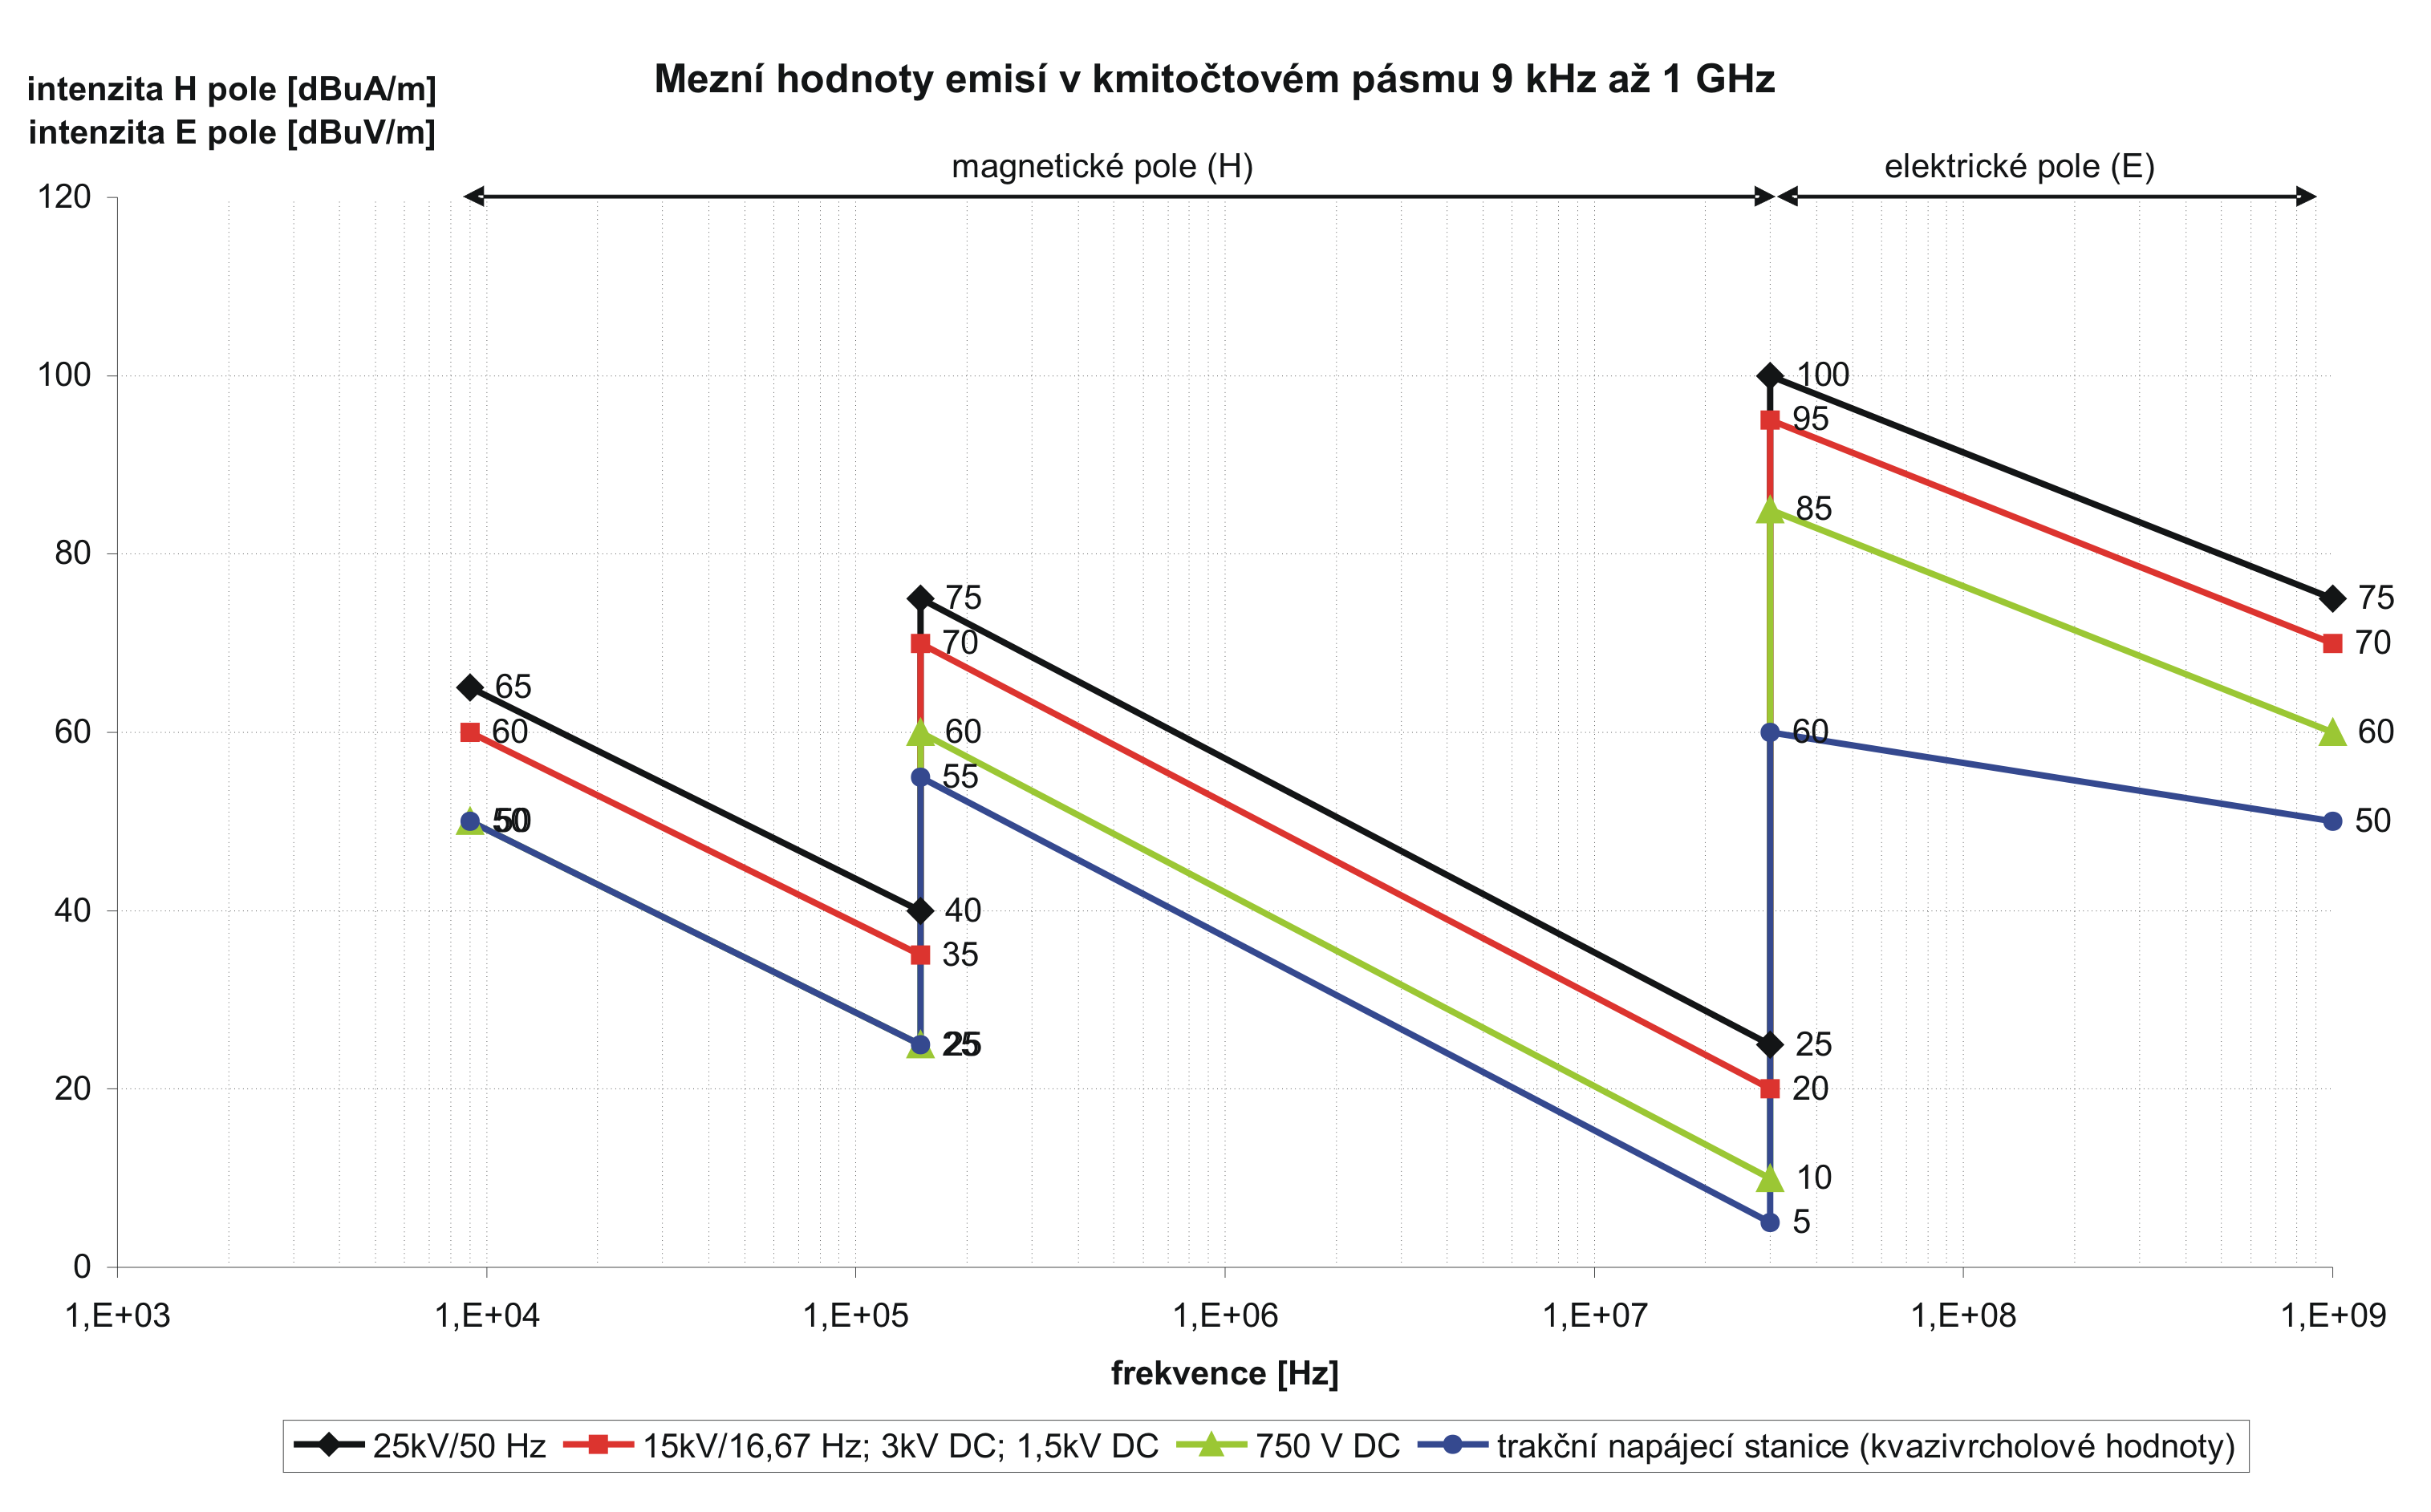
\includegraphics[width=12cm]{emc_emise2.png}
	\caption{Hranice emisí jednotlivých trakčních systémů.}
	\label{obr:emc_emise}
\end{figure}

Vlastní měření intenzity elektromagnetického pole, generovaného drážními vozidly, se provádí detektorem vrcholové hodnoty ve vzdálenosti 10 m od osy koleje. Určuje se horizontální magnetická složka pole (kolmá k~trati). U~elektrické složky vyzařovaného pole se měří složka vertikální a horizontální (rovnoběžná s~tratí). Normou definované šířky pásma pro pokles měřené veličiny o~6 dB  a použité měřící zařízení pro pokrytí celého kmitočtového pásma jsou uvedeny v~následující tabulce \ref{tab:emc_fr_rozsah}.

\begin{table}[!h]
\begin{center}
  	\caption{Přehled měřených frekvenčních rozsahů a měřících antén.}
  	\label{tab:emc_fr_rozsah}
\begin{tabular}{|l|l|l|l|}
	\hline
	{\bf Kmitočtový rozsah} & {\bf Pásmo} & {\bf Měřící anténa} & {\bf Měřená veličina} \\
	\hline
	\hline
	9 kHz - 150 kHz	& 200 Hz	& smyčková nebo rámová	& magnetická intenzita  H \\
	150 kHz - 30 MHz	& 9 kHz	& smyčková nebo rámová	& magnetická intenzita H \\
	30 MHz - 300 MHz	& 120 kHz	& bikónický dipól		& elektrická intenzita E \\
	300 MHz - 1 GHz	& 120 kHz	& logaritmicko - periodická	& elektrická intenzita E \\
  	\hline
\end{tabular}
\end{center}
\end{table}

\subsection{ČSN EN 50121-3-1}
Další platnou normou souboru Drážní zařízení – Elektromagnetická kompatibilita je ČSN EN 50121-3-1: Drážní vozidla – Vlak a celkové vozidlo. Týká se všech hnacích prostředků, včetně městských drah a ucelených vlakových souprav, ale rozsah platnosti této normy končí na rozhraní vozidla. Tím se rozumí buď kluzný kontakt s~trolejovým vedením nebo přívodní kolejnicí, případně konektor AC nebo DC napájení u~tažených vozidel. Předmětem této normy je stanovení zkušebních podmínek a mezí pro elektromagnetickou emisi a odolnost, aby tím bylo zajištěno fungování trakčního vozidla v~jeho definovaném prostředí. 

Zkoušky emisí jsou vykonávány při provozních stavech, při kterých se předpokládá nejvyšší produkovaná hodnota elektromagnetického rušení. Uvedené mezní hodnoty odpovídají emisím v~normě ČSN EN 50121-2, které jsou uvedeny na obrázku \ref{obr:emc_emise}.

Zkoušky odolnosti se neprovádějí, normou je pouze stanovena pevná hranice 20~V/m v~kmitočtovém rozsahu 0,15 MHz – 2 GHz , do které se považuje vozidlo za odolné.

\subsection{ČSN EN 50121-3-2}
Normativ ČSN EN 51231-3-2: Drážní vozidla – Zařízení definuje elektromagnetické poměry pro veškerá zařízení, které je možné používat na trakčním vozidle, tak aby bylo zajištěna bezproblémová činnost při všech provozních stavech. Je zde definována řada specifických požadavků. Například tato norma neplatí pro přechodné emise při vypnutí nebo zapnutí zařízení. Zvláštní požadavek platí pro prostředky radiokomunikací, pro které emise a odolnosti uvedené v~této normě neplatí. Pokud se jedná o~komponentu, kterou je potřeba připojit do systému vlastního vozidla, provádějí se veškeré zkoušky v~zapojeném stavu. Měření se navíc provádí pro všechny příslušné vstupy a výstupy. 
Rozlišují se na několik druhů, hlavní jsou uvedeny na obrázku \ref{obr:emc_IO}.

\begin{figure}[!h]
	\centering
	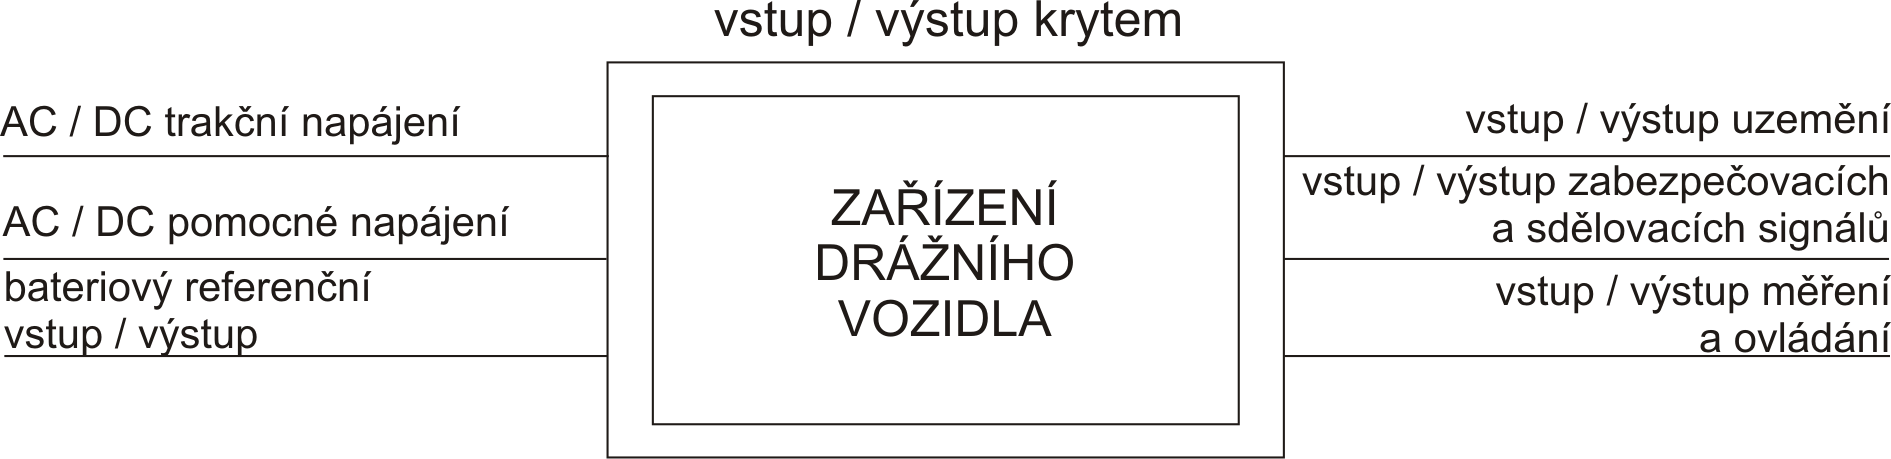
\includegraphics[width=8cm]{emc_IO.png}
	\caption{Hlavní druhy vstupů a výstupů zařízení.}
	\label{obr:emc_IO}
\end{figure}

Pro veškerá měřená zařízení se určují funkční kritéria, které jsou definované v~ČSN EN 50121-1, tj. A, B a C. Norma také definuje postup pro měření vysokofrekvenčního rušení přenášené po přívodním vedení v~pásmu 9 kHz až 30 MHz, které je vytvářeno především napájecími měniči trakčních motorů, obecně přístrojů se spínanými zdroji. Princip zkoušky je naznačen na obrázku \ref{obr:emc_vf}. 

\begin{figure}[!h]
	\centering
	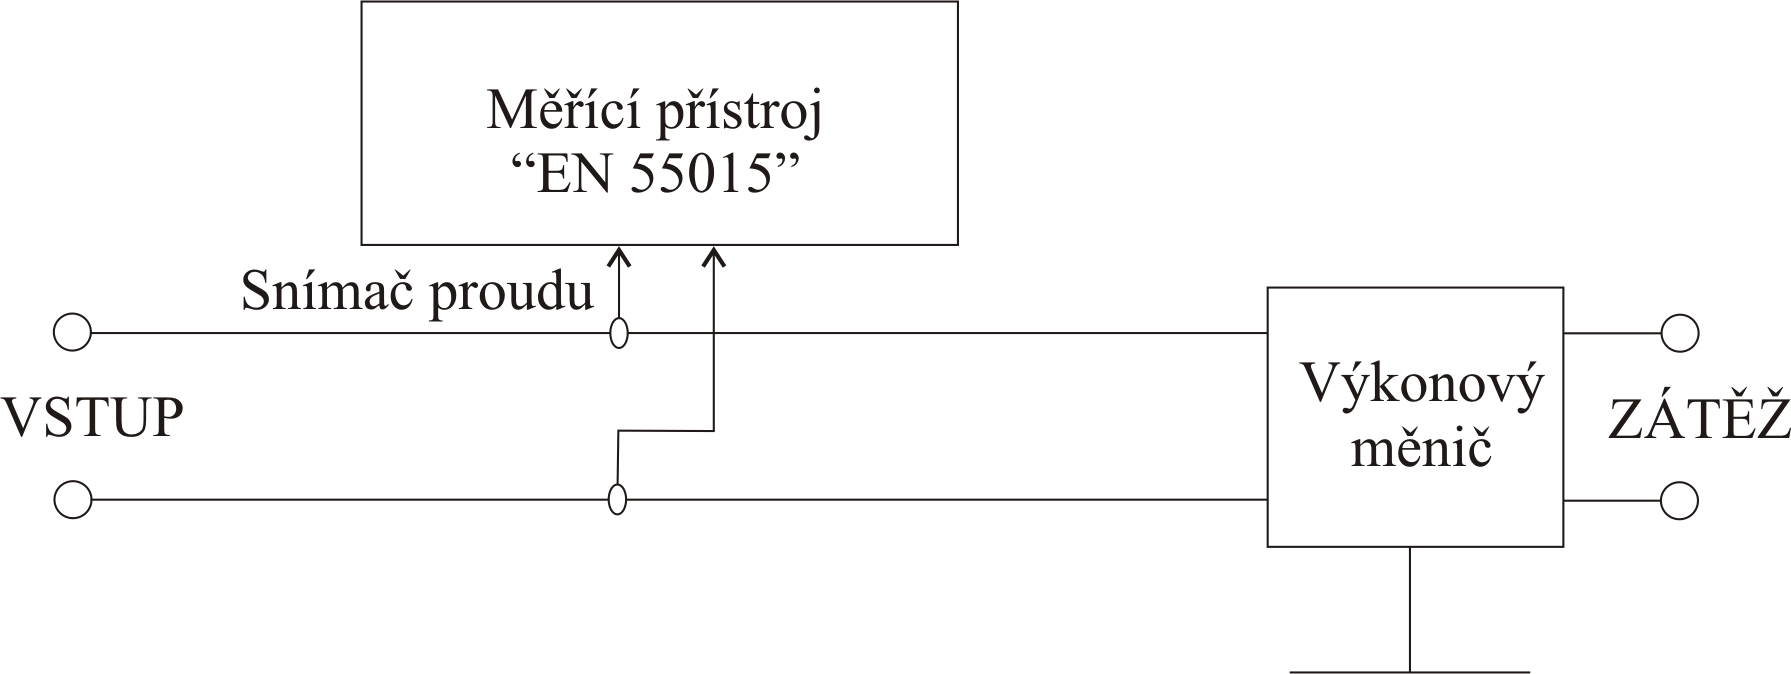
\includegraphics[width=8cm]{emc_vf.png}
	\caption{Hlavní druhy vstupů a výstupů zařízení.}
	\label{obr:emc_vf}
\end{figure}

Úrovně rušení se určují v~řadě měřících bodů po celé délce vedení a vyhodnocují se maximální rušivé proudy. Aby měření nebylo ovlivněno trakčním proudem, je potřeba zajistit správné impedanční přizpůsobení mezi snímačem proudu a měřícím přístrojem. Meze emisí pro rušení po vedení u~tohoto měření nastaveny nejsou, pokud se jedná o~samostatné zařízení. Pokud je instalování v~okolí jiného přístroje, musí vyhovovat mezním hodnotám vyzařování dle normy ČSN EN 50121-3-1.

Zkoušky odolnosti jsou touto normou specifikovány pro zkoušky postupného testování, v~libovolném pořadí. Popis metod a odkazy na základní normy pro vstupy a~výstupy krytem se nachází v~tabulce \ref{tab:emc_odolnosti1}.

\begin{table}[!h]
\catcode`\-=12
\begin{center}
  	\caption{Popis zkoušek odolnosti pro vstupy a výstupy krytem.}
  	\label{tab:emc_odolnosti1}
\begin{tabular}{|p{3,2cm}|p{2,8cm}|p{2,4cm}|p{2,3cm}|p{1,8cm}|}
	\hline
	{\bf\ Jevy prostředí} 	& \multicolumn{2}{c}{\bf Specifikace zkoušky}\vline & {\bf Základní norma} & {\bf Funkční kritérium} \\
	\hline
	\hline
	Vysokofrekvenční elektromagnetické pole (amplitudově modulované) & 80 - 1000 MHz 20 V/m (ef.) 80\% AM, 1kHz & Nemodulovaná nosná	& \begin{center}EN 61000-4-3 		\end{center}& \begin{center} A~\end{center} \\ 
	\hline
	 & 80 - 1000 MHz 20 V/m (ef.) 80\% AM, 1kHz & Nemodulovaná nosná &   &  \\
	\cline{2-3}
	Vysokofrekvenční elektromagnetické pole (digitální mobilní telefony) & 1400 - 1000 MHz 10 V/m (ef.) 80\% AM, 1kHz & Nemodulovaná nosná & 	\begin{center}  EN 61000-4-3  \end{center} & \begin{center} A~\end{center} \\
	\cline{2-3}
	& 2100 - 2500 MHz 5 V/m (ef.) 80\% AM, 1kHz & Nemodulovaná nosná	&  &  \\
	\hline
	Elektrostatický\linebreak[4]výboj & \begin{center} $\pm$6kV $\pm$8kV \end{center} & Kontaktní výboj \mbox{Vzduchový} výboj &\begin{center}EN 61000-4-2 \end{center} 
	& \begin{center}B\end{center} \\
	\hline
\end{tabular}
\end{center}
\end{table}

\begin{table}[!h]
\catcode`\-=12
\begin{center}
  	\caption{Další metody zkoušek odolnosti dle příšlušné normy.}
  	\label{tab:emc_odolnosti2}
\begin{tabular}{|p{3,2cm}|p{2,8cm}|p{2,4cm}|p{2,3cm}|p{1,8cm}|}
	\hline
	{\bf\ Jevy prostředí} 	& \multicolumn{2}{c}{\bf Specifikace zkoušky}\vline & {\bf Základní norma} & {\bf Funkční kritérium} \\
	\hline
	\hline
Vysokofrekvenční nesymetricky & 0,15 - 80~MHz 20~V~(ef.) 80~\%~AM, 1~kHz & Nemodulovaná nosná	& \begin{center}EN 61000-4-6 \end{center}& \begin{center} A~\end{center} \\ 
	\hline
Rychlé přechodné jevy & 5/50~$\mu$s 5~kHz $\pm$2~kV ($\pm$1~kV I/O uzemněním) ($\pm$4~kV pro I/O AC/DC)& Tr/Tn\linebreak[4]Kmitočet opakování Vrcholová & \begin{center}  EN 61000-4-4 \end{center} & \begin{center} A~B~pro~I/O \end{center} \\
	\hline
	Rázové impulsy & $\pm$~2 kV 42~$\Omega$ 0,5~$\mu$F 1,2/50~$\mu$s  & Zkuš. napětí naprázdno,\linebreak[4]mezi vodičemi a zemí & \begin{center}  EN 61000-4-5 \end{center} & \begin{center} B \end{center} \\
	\cline{2-3}
			& $\pm$~1 kV 42~$\Omega$ 0,5~$\mu$F 1,2/50~$\mu$s& Zkuš. napětí naprázdno,\linebreak[4]mezi vodiči &  &  \\
	\hline
\end{tabular}
\end{center}
\end{table}

Další specifika metod uvedená tabulce \ref{tab:emc_odolnosti2} jsou definovány pro následující vstupy a~výstupy:
\begin{itemize*}
\item vztahující se k~baterii  (s~výjimkou na výstupu zdrojů energie)
\item pomocné AC napájecí I/O
\item signálů a komunikací, měření a ovládání procesu
\item I/O DC napájení (ČSN EN 50121-4, 5)
\item I/O AC napájení (ČSN EN 50121-4, 5)
\item I/O uzemněním (ČSN EN 50121-4, 5)
\item I/O pro signálová vedení, datové sběrnice nezahrnuté do řízení (ČSN EN 50121-5)
\item I/O pro měřící a ovládací vedení, dlouhé sběrnice (ČSN EN 50121-5)
\end{itemize*}

\subsection{ČSN EN 50121-4}
Zjišťováním emisí a odolností zabezpečovacích a sdělovacích zařízení se týká další část, tj.~ČSN EN 50121-4. Tato norma se však zabývá pouze těmi přístroji, které jsou instalovány v~drážním prostředí mimo těch, které jsou umístěny v~trakčních vozidlech. Ty jsou pokryty ČSN EN 50121-3-2. 

Emise produkované zařízením, kterého se norma týká, musí splňovat maximální hodnoty uvedené ve všeobecné normě EN 61000-6-4. Specifika zkoušky jsou však uvedena zde, jedná se o~definování měřící vzdálenosti a případné přepočty výsledků vzhledem k~této vzdálenosti.

Z~hlediska odolnosti se používají funkční kritéria uvedená již v~ČSN EN 50121-1. Zkoušky se provádějí metodou postupného testování, jako jednotlivé zkoušky za sebou, viz. tabulka \ref{tab:emc_odolnosti1} a tabulka \ref{tab:emc_odolnosti2}.
 Měly by být prováděné při typických provozních režimech, kdy je uvažována maximální úroveň rušení v~daném frekvenčním rozsahu. Popis zkušebních metod není v~této normě uveden, je zde opět uveden odkaz na základní normy, zabývající se zkouškami odolnosti. 

\subsection{ČSN EN 50121-5}
Pro zajištění kompatibilní úrovně elektromagnetické emise a odolnosti pro elektrická a elektronická zařízení, určené k~použití v~pevných trakčních zařízení, je stanovena norma ČSN EN 50121-5. Zahrnuje  napájecí trakční stanice, prostředky s~obvody ochran, výkonové autotransformátory, zvyšovací transformátory a spínače pro dálkové i místní napájení. Filtry pracující v~napájecí síti, například pro kompenzaci účiníku, nejsou předmětem této normy,  pro ně jsou stanoveny jiné specifické požadavky. 

Norma definuje emise a odolnosti pro zařízení, která jsou umístěna uvnitř napájecí stanice nebo v~prostoru elektrifikované trati a případně i pro přístroje, které jsou napájené z~trakčního vedení, ale neslouží k~trakčním účelům. Konkrétně se jedná o~prostředky staniční služby (návěstní soustava), nádražní osvětlení, nakládací jeřáby a administrativní budovy.  

Emise se rozlišují na vyzařování z~vlastní trakční stanice do okolí a na generované uvnitř samotných napájecích stanic. Hranice záření do okolí jsou pro kmitočtové pásmo 9 kHz až 1 GHz stanoveny společně normou ČSB EN 50121-2. Pro zařízení umístěné pod zemí se musí provést měření v~rozsahu 9 kHz až 150 kHz v~prostoru na povrchu nad zařízením. Pokud se jedná o~venkovní nebo kabelová vedení mezi napájecí stanicí a~dráhou, není zde z~důvodu rozmanitosti možné stanovit mezní hodnoty pro magnetická pole, která vytvářejí. Ze stejného důvodu nejsou určeny meze pro rušení uvnitř trakčních napájecích stanic. 

Funkční kritéria jsou používány všeobecné, tzn. stejné jako jsou uvedené v~normě ČSN EN 50121-1. Pro zkoušky odolnosti platí to samé jako v~ČSN EN 50121-4, zkušební metody jsou uvedeny v~tabulkách \ref{tab:emc_odolnosti1} a \ref{tab:emc_odolnosti2}.
